%\renewcommand{\theequation}{\theenumi}
%\begin{enumerate}[label=\arabic*.,ref=\theenumi]
\begin{enumerate}[label=\thesection.\arabic*.,ref=\thesection.\theenumi]
\numberwithin{equation}{enumi}
	\item Let $\vec{D}_3, \vec{E}_3, \vec{F}_3$, be points on $AB, BC$ and $CA$ respectively such that
		\begin{align}
			BD_3 = BF_3=m, CD_3 = CE_3=n, AE_3 = AF_3=p.
		\end{align}
	Obtain $m,n,p$ in terms of $a,b,c$ obtained in  
		\probref{prob:side-length}.
 \\
 		\solution 
From the given information, 
\begin{align}
% 
    a &= m+n,\\
    b &= n+p, \\
    c &= m+p 
\end{align}
which can be expressed as
\begin{align}
\myvec{1&1&0\\0&1&1\\1&0&1\\}\myvec{m\\n\\p} &= \myvec{a\\b\\c}
\\
\implies 
	\myvec{m\\n\\p} &= \myvec{1&1&0\\0&1&1\\1&0&1\\}^{-1}\myvec{a\\b\\c}
\end{align}
Using row reduction,
		\begin{align}
			\augvec{3}{3}{1&1&0 & 1 & 0 & 0\\0&1&1 & 0 & 1 & 0\\1&0&1 & 0 & 0 & 1}
			\\
			\xleftrightarrow[]{R_3 \leftarrow R_3 - R_1}
			\augvec{3}{3}{1&1&0 & 1 & 0 & 0\\0&1&1 & 0 & 1 & 0\\0&-1&1 & -1 & 0 & 1}
			\\
			\xleftrightarrow[R_1 \leftarrow R_1 - R_2]{R_3 \leftarrow R_3 + R_2}
			\augvec{3}{3}{1&0&-1 & 1 & -1 & 0\\0&1&1 & 0 & 1 & 0\\0&0&2 & -1 & 1 & 1}
		\end{align}
		\begin{align}
			\xleftrightarrow[R_1 \leftarrow 2R_1 + R_3]{R_2 \leftarrow 2R_2 - R_3}
			\augvec{3}{3}{2&0&0 & 1 & -1 & 1\\0&2&0 & 1 & 1 & -1\\0&0&2 & -1 & 1 & 1}
		\end{align}
yielding
		\begin{align}
			\myvec{1&1&0\\0&1&1\\1&0&1\\}^{-1} = 
			\frac{1}{2}\myvec{1 & -1 & 1\\ 1 & 1 & -1\\ -1 & 1 & 1}
		\end{align}
	Therefore,
\begin{align}
\begin{split}
    p&=\frac{c+b-a}{2}
    =\frac{\sqrt{74}+\sqrt{32}-\sqrt{122}}{2}
    \\
    m&=\frac{a+c-b}{2}
    =\frac{\sqrt{74}+\sqrt{122}-\sqrt{32}}{2}
    \\
    n&=\frac{a+b-c}{2}
    =\frac{\sqrt{122}+\sqrt{32}-\sqrt{74}}{2}
\end{split}
	\label{eq:incircle-mnp}
\end{align}
upon substituting from 
		\eqref{eq:geo-norm-ab},
		\eqref{eq:geo-norm-bc}
		and
		\eqref{eq:geo-norm-ca}.

	\item Using section formula, find 
		\begin{align}
			\vec{D}_3 = \frac{m\vec{C}+n\vec{B}}{m+n},\,
			\vec{E}_3 = \frac{n\vec{A}+p\vec{C}}{n+p},\,
			\vec{F}_3 = \frac{p\vec{B}+m\vec{A}}{p+m}
		\end{align}
	\item Find the circumcentre and circumradius of $\triangle D_3E_3F_3$.  These are the {\em incentre} and {\em inradius} of $\triangle ABC$.
	\item Draw the circumcircle of $\triangle D_3E_3F_3$.  This is known as the {\em incircle} of $\triangle ABC$.
		\\
 		\solution
See 
	\figref{fig:incircle}
\begin{figure}[!ht]
	\centering
	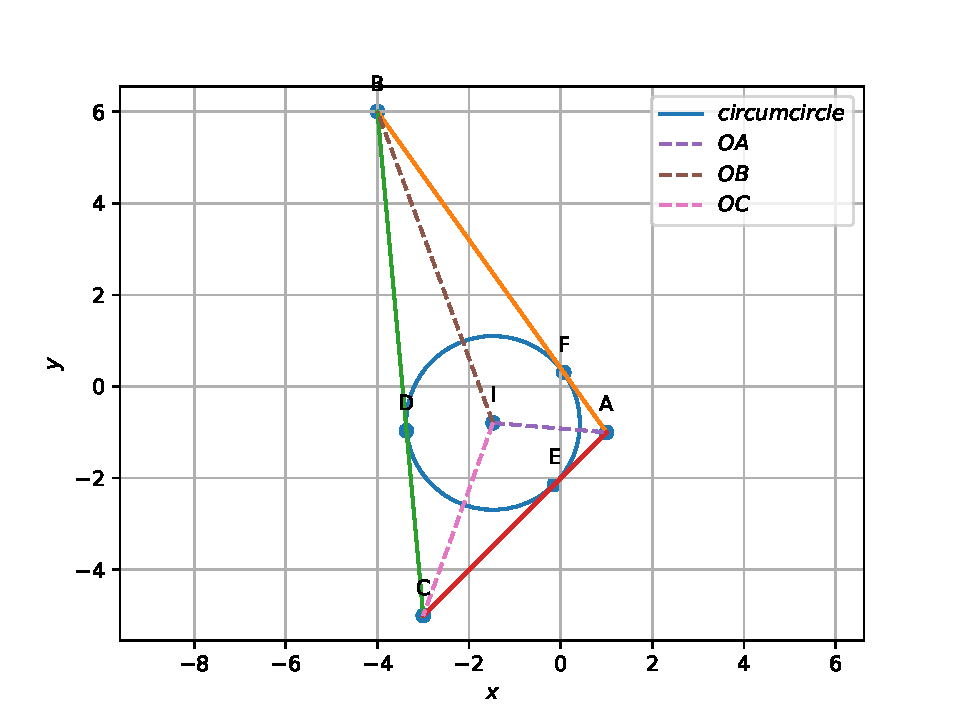
\includegraphics[width=\columnwidth]{figs/triangle/ang-bisect.pdf}
	\caption{Incircle of $\triangle ABC$}
	\label{fig:incircle}
\end{figure}
\iffalse
Considering
\begin{align}
	BC: \quad \vec{n} ^\top \vec{x} &= c, 
\end{align}
the distance from $\vec{I}$ to $BC$ is 
\begin{align}
\frac{\abs{\vec{n}^\top \vec{I} - c}}{\norm{\vec{n}}} 
\end{align}
\fi


	\item Using 
    \eqref{eq:angle2d}
verify that 
		\begin{align}
			\angle BAI = \angle CAI.
		\end{align}
		$AI$ is the bisector of $\angle A$.  
	\item Verify that $BI, CI$ are also the angle bisectors of $\triangle ABC$.

		\iffalse

\item Suppose the equations  given by 
		\begin{align}
			\label{eq:tri-sides}
			\vec{n}_i^{\top}\vec{x}=c_i \quad i = 1, 2, 3 
		\end{align}
		The equations of the respective angle bisectors are then given by 
		\begin{align}
			\frac{\vec{n}_i^{\top}\vec{x}-c_i}{\norm{\vec{n}_i}}
		=
	\pm	\frac{\vec{n}_j^{\top}\vec{x}-c_j}{\norm{\vec{n}_j}}
\quad i \ne j
		\end{align}
		Substitute numerical values and find the equations of the angle bisectors of $A, B$ and $C$.
	\\
		%\textbf{Solution :}
	The parametric equations of sides;
	\begin{align}
	BC:\quad &\myvec{11&1}\vec{x}=-38,\\
	CA:\quad &\myvec{1&-1}\vec{x}=2,\\
	AB:\quad &\myvec{7&5}\vec{x}=2\\	  
	\end{align}
	Using the formula mentioned in the question to find out the angular bisector for sides \text{AB} and \text{AC}, naming the angular bisector $L$ we get,
	\begin{align}
		\frac{\vec{n}_{3}^{\top} \vec{x}-c_{3}}{\norm{\vec{n}_{3}}}=\pm \frac{\vec{n}_{2}^{\top} \vec{x}-c_{2}}{\norm{\vec{n}_{2}}}
	\end{align}
	\begin{figure}
	\centering
	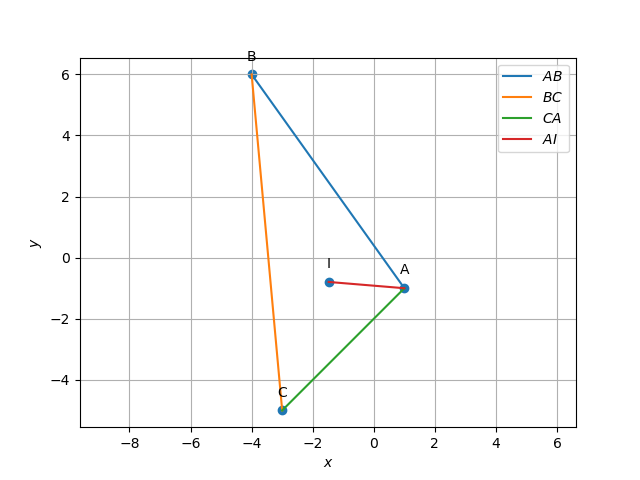
\includegraphics[width=\columnwidth]{solutions/1/5/1/figs/angular_bisector.png}
	\caption{Triangle generated using python}
	\label{fig:angular_bisector}
	\end{figure}
	As we can see we will get 2 solutions for $L$. This is because one of them is internal angular bisector and the other is the external angular bisector. Internal angular bisector can be evaluated if we take + in the above formula.
	Hence, $L$ is given by,
	\begin{align}
		\frac{\vec{n}_{3}^{\top} \vec{x}-c_{3}}{\norm{\vec{n}_{3}}}&=\frac{\vec{n}_{2}^{\top} \vec{x}-c_{2}}{\norm{\vec{n}_{2}}}\\
		\implies \brak{\frac{\vec{n_{3}}}{\norm{\vec{n_{3}}}}-\frac{\vec{n_{3}}}{\norm{\vec{n_{3}}}}} \vec{x}&=\brak{\frac{c_{3}}{\norm{\vec{n_{3}}}}-\frac{c_{2}}{\norm{\vec{n_{2}}}}}\\
		\implies \brak{\frac{\myvec{7&5}}{\sqrt{74}}-\frac{\myvec{1&-1}}{\sqrt{2}}} \vec{x}&=\frac{2}{\sqrt{74}}-\frac{2}{\sqrt{2}}\\
		\implies \myvec{\frac{7-\sqrt{37}}{\sqrt{74}}&\frac{5+\sqrt{37}}{\sqrt{74}}}\vec{x}&=\frac{2-2\sqrt{37}}{\sqrt{74}}
	\end{align}
	Hence, the internal angluar bisector of angle $A$, $L$ will be,
	\begin{align}
		\implies\myvec{\frac{7-\sqrt{37}}{\sqrt{74}}&\frac{5+\sqrt{37}}{\sqrt{74}}} \vec{x}=\frac{2-2\sqrt{37}}{\sqrt{74}}
		\label{eq:1.5.1}
	\end{align}
	

  \solution 
The above formula can 
be transformed to the normal equation of angle bisectors as  
\begin{align}
       \myvec{\frac{\vec{n}_i}{\norm{\vec{n}_i}} - \frac{\vec{n}_j}{\norm{\vec{n}_j}}}^{\top}\vec{x}
       =
       \frac{c_i}{\norm{\vec{n}_i}}-\frac{c_j}{\norm{\vec{n}_j}}
\end{align}
\begin{enumerate}
\item From 
		\eqref{eq:geo-norm-vec-ab}
		and 
		\eqref{eq:geo-norm-vec-ca}
the angle Bisector of $A$ is 
\begin{align}
\myvec{
\frac{7}{\sqrt{74}}-\frac{1}{\sqrt{2}} & \frac{5}{\sqrt{74}}+\frac{1}{\sqrt{2}}\\
}
\vec{x}
=\frac{2}{\sqrt{74}}-\frac{2}{\sqrt{2}}
\end{align}
\item Similarly, the angle bisector of $B$ is 
\begin{align}
\myvec{
\frac{11}{\sqrt{122}}+\frac{7}{\sqrt{74}} & \frac{1}{\sqrt{122}}+\frac{5}{\sqrt{74}}\\
}
\vec{x}
=\frac{2}{\sqrt{74}}-\frac{38}{\sqrt{122}}
\end{align}
\item and the angle bisector of $C$ is 
\begin{align}
\myvec{
\frac{11}{\sqrt{122}}+\frac{1}{\sqrt{2}} & \frac{1}{\sqrt{122}}-\frac{1}{\sqrt{2}}\\
}
\vec{x}
=\frac{2}{\sqrt{2}}-\frac{38}{\sqrt{122}}
\end{align}
\end{enumerate}

	\item Find the intersection $\vec{I}$ of the angle bisectors of $B$ and $C$.
	\item Find the distance from $\vec{I}$ to $BC$.  
  \\
		\solution
See 
	\figref{fig:incircle}
\begin{figure}[!ht]
	\centering
	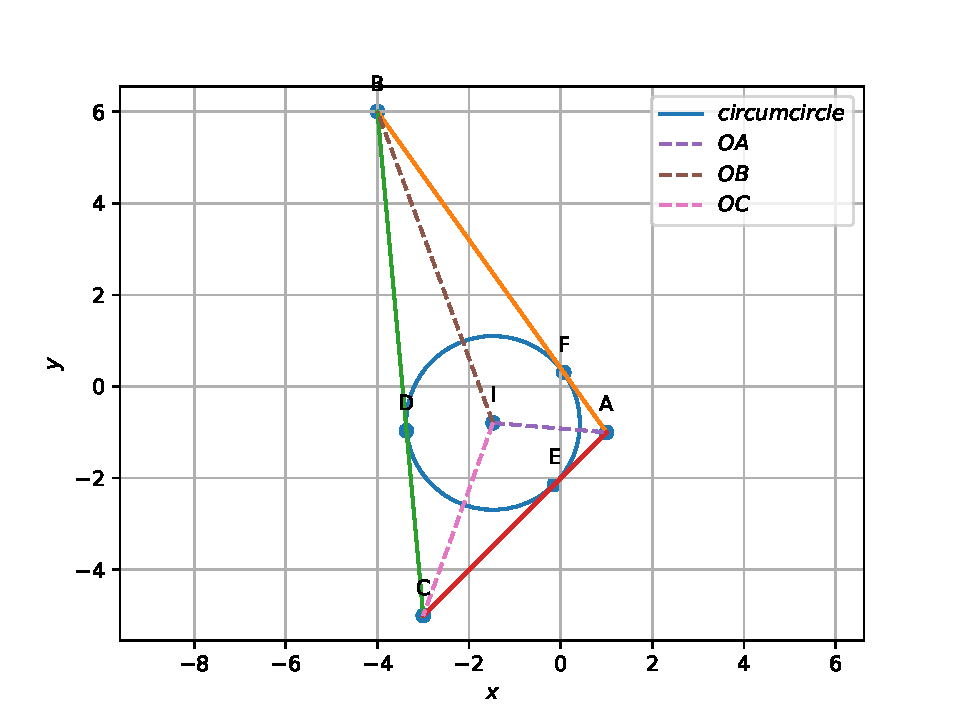
\includegraphics[width=\columnwidth]{figs/triangle/ang-bisect.pdf}
	\caption{Incircle of $\triangle ABC$}
	\label{fig:incircle}
\end{figure}
\iffalse
Considering
\begin{align}
	BC: \quad \vec{n} ^\top \vec{x} &= c, 
\end{align}
the distance from $\vec{I}$ to $BC$ is 
\begin{align}
\frac{\abs{\vec{n}^\top \vec{I} - c}}{\norm{\vec{n}}} 
\end{align}
\fi

 
	\item Repeat the above exercise for the sides $AB$ and $AC$.
	This distance is known as the {\em inradius} $r$.
	\item Draw a circle with center $\vec{I}$ and radius $r$.  $\vec{I}$ is known as the {\em incentre}.
	\item The equation of the {\em incircle} is given by 
		\begin{align}
			\label{eq:incircle}
			\norm{\vec{x}-\vec{I}}^2 = r^2
		\end{align}
		Using the parameteric equation of $BC$, verify that $BC$ intersects the incircle at exactly one point. $BC$ is defined to be a {\em tangent} to the incircle.
		\\
		\solution
Let 
\begin{align}
\vec{x} &= \vec{B} + k{\vec{m}}\label{eq:8}
\end{align}
Substituting \eqref{eq:8} in \eqref{eq:incircle}
\begin{align}
  \norm{ \vec{B} + k{\vec{m}}- \vec{I} }^2 &= r^2 \\
\implies   \brak{\vec{B} + k{\vec{m}}- \vec{I}}^{\top} \brak{\vec{B} + k{\vec{m}}- \vec{I}} &= r^2 
\\
	\text{or, }
	k^2\norm{\vec{m}}^2 +2k{\vec{m}^{\top}}\brak{{\vec{B}-\vec{I}}}+\norm{\vec{B}-\vec{I}}^2 &= 0
	\label{eq:incircle-disc}
\end{align}
It can be easily verified that 
\begin{align}
\cbrak{2\vec{m}^{\top}\brak{\vec{B}-\vec{I}}}^2
= 
	\norm{\vec{m}}^2\norm{\vec{B}-\vec{I}}^2
\end{align}
which implies that the discriminant of 
	\eqref{eq:incircle-disc}
	is 0.  Thus, BC intersects the circle at only one point.


	\item Find the {\em point of contact} $\vec{D}_3$ where $BC$ touches the incircle.
		\\
		\solution
Since
	\eqref{eq:incircle-disc}
	has only one root, 
\begin{align}
k=-\frac{\vec{m}^{\top}\brak{\vec{B}-\vec{I}}}{{\ \norm{\vec{m}}^2}}
\end{align}
Substituing the above in 
\eqref{eq:8},
\begin{align}
	\vec{D_{3}} = \vec{B} -\frac{\vec{m}^{\top}\brak{\vec{B}-\vec{I}}}{{\ \norm{\vec{m}}^2}} \vec{m}
\end{align}



  \item Find the other points of contact $\vec{E}_3$ and $\vec{F}_3$.
  \\
		\iffalse
\documentclass[journal,12pt,twocolumn]{IEEEtran}
\usepackage{cite}
\usepackage{amsmath,amssymb,amsfonts,amsthm}
\usepackage{algorithmic}
\usepackage{graphicx}
\usepackage{textcomp}
\usepackage{xcolor}
\usepackage{txfonts}
\usepackage{listings}
\usepackage{enumitem}
\usepackage{mathtools}
\usepackage{gensymb}
\usepackage[breaklinks=true]{hyperref}
\usepackage{tkz-euclide} % loads  TikZ and tkz-base
\usepackage{listings}
\usepackage{floatrow}  


\newtheorem{theorem}{Theorem}[section]
\newtheorem{problem}{Problem}
\newtheorem{proposition}{Proposition}[section]
\newtheorem{lemma}{Lemma}[section]
\newtheorem{corollary}[theorem]{Corollary}
\newtheorem{example}{Example}[section]
\newtheorem{definition}[problem]{Definition}
%\newtheorem{thm}{Theorem}[section] 
%\newtheorem{defn}[thm]{Definition}
%\newtheorem{algorithm}{Algorithm}[section]
%\newtheorem{cor}{Corollary}
\newcommand{\BEQA}{\begin{eqnarray}}
\newcommand{\EEQA}{\end{eqnarray}}
\newcommand{\define}{\stackrel{\triangle}{=}}
\theoremstyle{remark}
\newtheorem{rem}{Remark}

%\bibliographystyle{ieeetr}
\begin{document}
%


\providecommand{\pr}[1]{\ensuremath{\Pr\left(#1\right)}}
\providecommand{\prt}[2]{\ensuremath{p_{#1}^{\left(#2\right)} }}        % own macro for this question
\providecommand{\qfunc}[1]{\ensuremath{Q\left(#1\right)}}
\providecommand{\sbrak}[1]{\ensuremath{{}\left[#1\right]}}
\providecommand{\lsbrak}[1]{\ensuremath{{}\left[#1\right.}}
\providecommand{\rsbrak}[1]{\ensuremath{{}\left.#1\right]}}
\providecommand{\brak}[1]{\ensuremath{\left(#1\right)}}
\providecommand{\lbrak}[1]{\ensuremath{\left(#1\right.}}
\providecommand{\rbrak}[1]{\ensuremath{\left.#1\right)}}
\providecommand{\cbrak}[1]{\ensuremath{\left\{#1\right\}}}
\providecommand{\lcbrak}[1]{\ensuremath{\left\{#1\right.}}
\providecommand{\rcbrak}[1]{\ensuremath{\left.#1\right\}}}
\newcommand{\sgn}{\mathop{\mathrm{sgn}}}
\providecommand{\abs}[1]{\left\vert#1\right\vert}
\providecommand{\res}[1]{\Res\displaylimits_{#1}} 
\providecommand{\norm}[1]{\left\lVert#1\right\rVert}
%\providecommand{\norm}[1]{\lVert#1\rVert}
\providecommand{\mtx}[1]{\mathbf{#1}}
\providecommand{\mean}[1]{E\left[ #1 \right]}
\providecommand{\cond}[2]{#1\middle|#2}
\providecommand{\fourier}{\overset{\mathcal{F}}{ \rightleftharpoons}}
\newenvironment{amatrix}[1]{%
  \left(\begin{array}{@{}*{#1}{c}|c@{}}
}{%
  \end{array}\right)
}
%\providecommand{\hilbert}{\overset{\mathcal{H}}{ \rightleftharpoons}}
%\providecommand{\system}{\overset{\mathcal{H}}{ \longleftrightarrow}}
	%\newcommand{\solution}[2]{\textbf{Solution:}{#1}}
\newcommand{\solution}{\noindent \textbf{Solution: }}
\newcommand{\cosec}{\,\text{cosec}\,}
\providecommand{\dec}[2]{\ensuremath{\overset{#1}{\underset{#2}{\gtrless}}}}
\newcommand{\myvec}[1]{\ensuremath{\begin{pmatrix}#1\end{pmatrix}}}
\newcommand{\mydet}[1]{\ensuremath{\begin{vmatrix}#1\end{vmatrix}}}
\newcommand{\myaugvec}[2]{\ensuremath{\begin{amatrix}{#1}#2\end{amatrix}}}
\providecommand{\rank}{\text{rank}}
\providecommand{\pr}[1]{\ensuremath{\Pr\left(#1\right)}}
\providecommand{\qfunc}[1]{\ensuremath{Q\left(#1\right)}}
	\newcommand*{\permcomb}[4][0mu]{{{}^{#3}\mkern#1#2_{#4}}}
\newcommand*{\perm}[1][-3mu]{\permcomb[#1]{P}}
\newcommand*{\comb}[1][-1mu]{\permcomb[#1]{C}}
\providecommand{\qfunc}[1]{\ensuremath{Q\left(#1\right)}}
\providecommand{\gauss}[2]{\mathcal{N}\ensuremath{\left(#1,#2\right)}}
\providecommand{\diff}[2]{\ensuremath{\frac{d{#1}}{d{#2}}}}
\providecommand{\myceil}[1]{\left \lceil #1 \right \rceil }
\newcommand\figref{Fig.~\ref}
\newcommand\tabref{Table~\ref}
\newcommand{\sinc}{\,\text{sinc}\,}
\newcommand{\rect}{\,\text{rect}\,}
%%
%	%\newcommand{\solution}[2]{\textbf{Solution:}{#1}}
%\newcommand{\solution}{\noindent \textbf{Solution: }}
%\newcommand{\cosec}{\,\text{cosec}\,}
%\numberwithin{equation}{section}
%\numberwithin{equation}{subsection}
%\numberwithin{problem}{section}
%\numberwithin{definition}{section}
%\makeatletter
%\@addtoreset{figure}{problem}
%\makeatother

%\let\StandardTheFigure\thefigure
\let\vec\mathbf


\bibliographystyle{IEEEtran}


\vspace{3cm}

\title{
%	\logo{
Assignment 1
%	}
}
\author{ EE22BTECH11053 - Tanmay Vishwasrao% <-this % stops a space
	
}	

\maketitle

\newpage

%\tableofcontents

\bigskip

\renewcommand{\thefigure}{\theenumi}
\renewcommand{\thetable}{\theenumi}
Question 1.5.9\\
Find the other points of contact $\vec{E}_3$ and $\vec{F}_3$.
\fi
\solution
From the previous references we have the value of Incentre $\vec{I}$ is
\begin{align}
\vec{I} &=\myvec{-1.4775\\-0.7949}
\end{align}
And the value of inradius $r$ is 1.8969. The parametric equation of line is:
\begin{align}
&= \vec{A}+k\vec{m}
\end{align}
The equation of Incircle is given by:
\begin{align}
\norm{\vec{x}-\vec{I}}^2 &= r^2
\end{align}
Since its a parametric equation we can substitute $(3)$ as $\vec{x}$ in $(4)$.
\begin{align}
\norm{\vec{A}+k\vec{m}-\vec{I}}^2 &= r^2 \\
\brak{\vec{A}+k\vec{m}-\vec{I}}^\top\brak{\vec{A}+k\vec{m}-\vec{I}} &= r^2
\end{align}
On simplifying the above equation:
\begin{align}
k^2\norm{\vec{m}}^2+2k\brak{\vec{m}}^\top\brak{\vec{A-I}}+\norm{\vec{I}}^2 \nonumber \\
+\norm{\vec{A}}^2-2\brak{\vec{A}^\top\vec{I}}-r^2 &= 0 \label{eq:equation8721}
\end{align}
\begin{enumerate}
\item Finding the point $\vec{E}_3$.\\
The equation of $\vec{E}_3$:
\begin{align}
\vec{E}_3 &=\vec{A}+k\vec{m}
\end{align}
Where 
\begin{align}
\vec{m} = \vec{A}-\vec{B}
\end{align}
Now putting the values of $\vec{A}, \vec{m}, \vec{I}$ in \eqref{eq:equation8721}.
\begin{align}
74k^2+27.6463k+2.5821 &= 0
\end{align}
Discriminant of the above equation is:
\begin{align}
D &= \brak{27.6463}^2-4\brak{74}\brak{2.5821}\\
&= 764.3179-764.3179\\
&= 0
\end{align}
Since the discriminant is $0$. The value of k will be:
\begin{align}
k &= -\frac{2\brak{\vec{m}}^\top\brak{\vec{A-I}}}{2\norm{\vec{m}}^2} \\
&= -\frac{27.6463}{148} \\
&= -0.1867
\end{align}
Now we can find $\vec{E}_3$ using above results:
\begin{align}
\vec{E}_3 &=\myvec{1\\-1}-0.1867\myvec{5\\-7} \\
&=\myvec{0.066\\0.307}
\end{align}
\item Finding the point $\vec{F}_3$.\\
For the point $\vec{F}_3$ the value of $\vec{m} = \vec{A}-\vec{C}$. 
\begin{align}
\vec{F}_3 &=\vec{A}+k\vec{m}
\end{align}
Now putting the values of $\vec{A}, \vec{m}, \vec{I}$ in \eqref{eq:equation8721}.
\begin{align}
32k^2+18.1801k+2.5821 &= 0
\end{align}
Discriminant of the above equation is:
\begin{align}
D &= \brak{18.1801}^2-4\brak{32}\brak{2.5821}\\
&= 330.51-330.51\\
&= 0
\end{align}
Since the discriminant is $0$. The value of k will be:
\begin{align}
k &= -\frac{2\brak{\vec{m}}^\top\brak{\vec{A-I}}}{2\norm{\vec{m}}^2}\\
&= -\frac{18.1801}{64}\\
&= -0.2840
\end{align}
Now we can find $\vec{F}_3$ using above results:
\begin{align}
\vec{F}_3 &=\myvec{1\\-1}-0.2840\myvec{4\\4}\\
&= \myvec{-0.136\\-2.136}
\end{align}
\end{enumerate}
\iffalse
\begin{figure}[H]
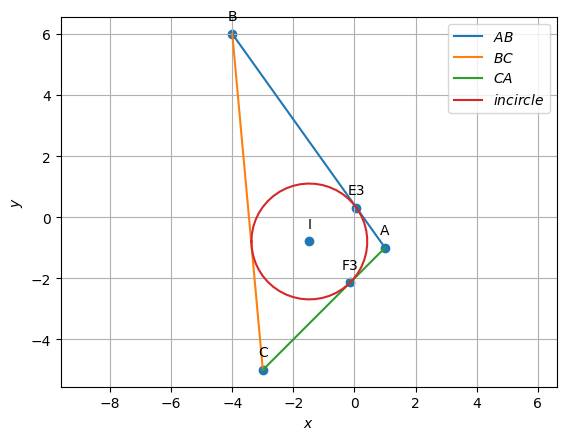
\includegraphics[width=\columnwidth]{solutions/1/5/9/figs/Incircle.png}
\caption{Points $\vec{E}_3$ and $\vec{F}_3$ plotted using python}
\label{fig:i_tri_py_1_5_9}
\end{figure}
\fi


		\fi
\end{enumerate}
